\section{Dataset} \label{sec:chp5-sec4}

%This section describes the acquired polarimetric dataset.
%The first prototype 
This polarimetry dermoscope prototype has been tested in the Melanoma Unit of the Clinic Hospital of Barcelona during the past three years.
In this time, series of polarimetry images of over 200 lesions were acquired.
Due to focusing issues, some images had to be discarded, and, as a result, only 197 lesions were considered. 
In this set, 56 lesions were provided with a histopathology conclusion and 141 were assumed benign without histopathology.
From the lesions for which a biopsy was performed, 22 were melanoma and 34 were classified either as dysplastic nevus, keratosis, basal cell carcinoma or benign lesions.
Table~\ref{tab:table1} lists the total number of different lesion types.
\begin{table}
	\caption[Summary of acquired polarimetric dataset]{Summary of the polarimetric dataset acquired with the prototype.}
	\centering
		\begin{tabular}{l c c}
		\toprule
		Lesion & Histopathology & \# Samples\\
		\midrule
		Melanoma & $\checkmark$ & 22\\
		Dysplastic & $\checkmark$ & 19\\
		Basel cell carcinoma & $\checkmark$ & 3\\
		Keratosis & $\checkmark$ & 4\\
		\multirow{2}{*}{Benign} & $\checkmark$ & 8 \\
		& - & 141 \\
		\bottomrule
		\end{tabular}
	\label{tab:table1}
\end{table}
\clearpage
\section{Methodology} \label{sec:chp5-sec5}

Figure~\ref{fig:PD-Framework} shows our proposed framework for the automatic classification of melanoma lesions using polarized images. 
Similar to the framework for dermoscopy images (see Fig.\,\ref{fig:dermoscopyFramework}), this framework is also composed of 6 main steps: pre-processing, mapping, feature extraction, representation, balancing and classification.
These steps are explained in the following. 
%\tikzstyle{decision} = [diamond, draw, fill=blue!20, 
%    text width=4.5em, text badly centered, node distance=3cm, inner sep=0pt]
\tikzstyle{block} = [rectangle, draw, fill= blue!30, text = black, 
   text width=7em, text centered, rounded corners, minimum height=4em , minimum width = 7em]
\tikzstyle{block2} = [rectangle, draw, fill=white!20,
    text width=7em, text centered, rounded corners, minimum height=4em, minimum width = 7em]
\tikzstyle{block3} = [rectangle, draw, fill=blue!30,
    text width=7em, text centered, rounded corners, minimum height=3em , minimum width = 7em]
\tikzstyle{myarrow}=[->, thick]
\tikzstyle{myarrow2}=[dashed, ->, thick]
\tikzstyle{line}=[-, thick]
\def\blockdist{1}
\def\edgedist{1.5}
 
\begin{figure}
\begin{center}   
\begin{tikzpicture}[node distance = 1cm,scale=0.7, every node/.style={scale=0.7}]
    % Place nodes
    %\node [block] (init) {initialize model};
    \node [block2] (input) {$I_{0}$, $I_{45}$, $I_{90}$};
    	\path (input.east|- input.south)+(+0.1,1.5) node (a) {};
	\path (input.west)+(0.04,0) node (b) {}; 
	%\node[block, right of=a , node distance =2.35cm](Reg){Registration};
	\node[block, right of=a, node distance = 2.3cm] (S3){I,Q,U}; 
	\node[block, above of = S3, node distance = 1.7 cm](Reg){Registration}; 
	%\node[block, below of = Reg, node distance = 1.7 cm](S3){I,Q,U}; 
    \node[block, below of = S3, node distance = 1.7cm ](HR){Hair removal};
    \node[block, below of = HR, node distance = 1.7 cm] (Seg){Segmentation}; 
    	\path (Reg.south|- S3.north)+(2,0) node (c) {};
	\path (HR.south|- Seg.north)+(2,0) node (m) {}; 
	\node[block, right of = input, node distance = 7.3cm](Map){Global Mapping}; 
	\node[block, right of = c, node distance = 5.1cm](PF){Polarized features}; 
	\node[block, below of = PF, node distance = 2.8cm](SF){Spatial features};
	\node[block, right of = Map, node distance = 7.5cm](LR){Low representation}; 
	
	
	\node[block, below of = LR, node distance = 5cm](US){Under-sampling};  
	\node[block, below of = US, node distance = 2.8cm](OS){Over-sampling}; 
	\path(US.south|- OS.north)+(-1.6,0.4) node (l){}; 
	\node[block, left of = l, node distance = 2.5cm](Cls) {Classification}; 
	    
    %\node[block, right of = input, node distance = 15.5cm](Cls){Ensemble}; 
    
    \begin{pgfonlayer}{background}
	\path (Reg.west |- Reg.north)+(-0.4,\blockdist) node (d) {};
    \path (Seg.east |- Seg.south)+(+0.4,-0.5) node (e) {};          
    \path[fill=blue!10,rounded corners, draw=blue!20, dashed] (d) rectangle (e);
	\end{pgfonlayer}
	\path (Reg.west |- Reg.north) +(+1.4,-0.5+\blockdist) node (PRE) {\textbf{Pre-processing}};
	
 	\begin{pgfonlayer}{background}
	\path (Reg.west |- Reg.north)+(6.7,\blockdist) node (d) {};
    \path (Seg.east |- Seg.south)+(+7.5,-0.5) node (e) {};          
    \path[fill=blue!10,rounded corners, draw=blue!20, dashed] (d) rectangle (e);
	\end{pgfonlayer}
	\path (Reg.west |- Reg.north) +(+8.5,-0.5+\blockdist) node (FE) {\textbf{Feature extraction}};
	
    \begin{pgfonlayer}{background}
	\path (US.west |- US.north)+(-0.4,0.8+\blockdist) node (d) {};
    \path (OS.east |- OS.south)+(+0.4,-1.9) node (e) {};          
    \path[fill=blue!10,rounded corners, draw=blue!20, dashed] (d) rectangle (e);
	\end{pgfonlayer}
	\path (US.west |- US.north) +(+1.4,+0.3+\blockdist) node (Bal) {\textbf{Balancing}};
	
	
	
% 	\begin{pgfonlayer}{background}
%	\path (Reg.west |- Reg.north)+(7.5,\blockdist) node (d) {};
%    \path (HR.east |- HR.south)+(+8.3,-0.5) node (e) {};          
%    \path[fill=blue!10,rounded corners, draw=blue!20, dashed] (d) rectangle (e);
%	\end{pgfonlayer}
%	\path (Reg.west |- Reg.north) +(+9.2,-0.5+\blockdist) node (Bal) {\textbf{Balancing}};
%	
%	\begin{pgfonlayer}{background}
%	\path (Reg.west |- Reg.north)+(11.4,\blockdist) node (d) {};
%    \path (HR.east |- HR.south)+(+12.2,-0.5) node (e) {};          
%    \path[fill=blue!10,rounded corners, draw=blue!20, dashed] (d) rectangle (e);
%	\end{pgfonlayer}
%	\path (Reg.west |- Reg.north) +(+13.0,-0.5+\blockdist) node (Bal) {\textbf{Classification}};
%	

%    \begin{pgfonlayer}{background}
%	\path (PF.west |- PF.north)+(-0.4,+1.0\blockdist) node (d) {};
%    \path (SF.east |- SF.south)+(+0.4,-2.0) node (e) {};          
%    \path[fill=blue!10,rounded corners, draw=blue!20, dashed] (d) rectangle (e);
%	\end{pgfonlayer}
%	\path (PF.west |- PF.north) +(+1.4,-0.5+\blockdist) node (FE) {\textbf{Feature extraction}};
	
%	\begin{pgfonlayer}{background}
%	\path (PF.west |- PF.north)+(3.5,\blockdist) node (d) {};
%    \path (SF.east |- SF.south)+(4.3,-0.5) node (e) {};          
%    \path[fill=blue!10,rounded corners, draw=blue!20, dashed] (d) rectangle (e);
%	\end{pgfonlayer}
%	\path (PF.west |- PF.north) +(+5.3,-0.5+\blockdist) node (FEs) {\textbf{Balancing}};
	
%	\begin{pgfonlayer}{background}
%	\path (PF.west |- PF.north)+(7.4,\blockdist) node (d) {};
%    \path (SF.east |- SF.south)+(8.2,-0.5) node (e) {};          
%    \path[fill=blue!10,rounded corners, draw=blue!20, dashed] (d) rectangle (e);
%	\end{pgfonlayer}
%	\path (PF.west |- PF.north) +(9.2,-0.5+\blockdist) node (cls1) {\textbf{Classification}};

	\path (input.east) + (0.8,0) node (f) {}; 
	\path (input.east) + (4.0,0) node (g) {};
	\path (input.east) + (4.8,0) node (h) {};
        \path (input.east) + (7.9,0) node (i) {};
	\path (input.east) + (11.2,0)node (j) {};
	\path (LR.south)   + (0,-1.9) node (k) {}; 
	
	
%	\path (input.east) + (11.9,0) node (k) {};
%	\path (input.east) + (12.6,0) node (l) {};

	
	\draw [myarrow] (input) -- (f); 
	\draw [myarrow] (g) -- (Map); 
	\draw [myarrow] (Map) --(i); 
    \draw [myarrow] (j) -- (LR); 
    \draw [myarrow] (LR) --(k) ; 
    \draw [myarrow] (l) --(Cls); 
    %\draw [myarrow] (k) -- (l); 



\end{tikzpicture}
\end{center}
\caption{Proposed framework for automatic classification of melanoma lesions based on polarimetric images.}
\label{fig:PD-Framework}
\end{figure}




%---------------------
\subsection{Pre-processing}
%This section contains the necessary steps prior to mapping and feature extraction steps.
For each lesion, three polarized images are acquired using the device proposed.
As mentioned above, the polarizer in the \ac{psa} unit rotates automatically during the image acquisition, so the quality and accuracy of the images in terms of polarization angles is ensured.
However, since the device is positioned and focused manually during the acquisition process, the images may be out of focus and/or misaligned.
When there is a focusing problem, the images are simply excluded from the dataset, whereas in the case of misalignment, the images must undergo a registration procedure.
%The images with the former problem, out of focus, are excluded from the dataset, while the ones with registration problem are registered prior to any processing.
Then the registered images are processed to acquire the first Stokes parameters, I, Q, and U (see Sect.~\ref{sec:chp5-sec3}), and to remove any artifacts.
Finally, the combination of the new triplet images and the acquired images is used for lesion segmentation.
%However prior to segmentation, the artifacts such as hairs are removed using our proposed hair removal algorithm.
%We use our proposed hair removal algorithm to remove the hairs and then combination of the new triplet images and the acquired images are used for segmentation.
All these stages are explained below.

\subsubsection{Registration}

Image registration is a crucial step prior to further processing: for optimal polarimetric measurements, the intensities retrieved from all the images must correspond to the same spatial locations.
%For the sake of optimal polarized measurements, the intensities retrieved from all polarimetric images should correspond to the same spatial locations.
Thus, the three acquired images should be perfectly aligned.

Image registration uses geometric transformations to align an unregistered image (moved image) to the reference image (fixed image).
In this research, we consider the second acquired image $I_{\ang{45}}$ as the fixed image (reference image), so the first and third images are registered onto this reference.
The registration is performed by means of a transformation model that relates the unregistered image to the reference frame.
Rigid (affine) and non-rigid, or elastic, transformations are two common transformation models. 
The transformation model required here should preserve the shapes and borders of the lesion without deforming it.
These criteria is required to preserve the intrinsic criteria of the lesions with the assumption that they have not been deformed in the acquisition process.
In this regard, affine rigid transformation is opted since it preserves the ratios of distances and angles (thanks to its linearity).
%We opted for the affine rigid transformation model in this work because, thanks to its linearity, it preserves the ratios of distances and angles.

%furthermore transformation of the edges and the shape of the lesions are not desirable.
%A rigid transformation in 2-D has three degrees of freedom: translation, rotation and scaling.
%Here rigid transformation which involves translation, rotation and scaling as the basic three transformations is used.
Thus, our registration framework consists of four main steps: (i) feature detection, (ii) feature matching, (iii) mapping estimation, and (iv) image transformation~\cite{zitova2003image}.

\begin{description}
	\item[Feature detection] refers to the detection of distinct aspects of each image such as corners, closed boundaries, line intersections, and highly textured patches.
	Different detectors, such as Harris, Hessian, \ac{sift}, or \ac{surf}, are used for finding salient and distinct points in images.
	Once the feature locations are known, different descriptors can be used for their unique representation, e.g. \ac{sift} or \ac{surf}~\cite{bay2006surf}.	
	
	\item[Feature matching] refers to establishing correspondences between features detected in the unregistered and reference images.
	Feature descriptors are usually matched based on similarity measurements such as correlation or distance ratio.
	
	\item[Mapping estimation] provides a mapping function that transforms the unregistered image to the fixed image frame.
	The parameters of the mapping function (e.g., homography) are calculated based on the feature correspondences from the previous step~\cite{zitova2003image}.
	
	\item[Image transformation] serves to actually transform the unregistered image to the reference frame based on the mapping function estimated in the previous step.
\end{description}

In this work, \ac{surf} was used for feature detection and description, correlation was employed as the similarity measure, and the mapping function (homography) was built as an affine transformation between corresponding feature points.
Finally, using the estimated rigid (affine) transformation, the unregistered $I_{\ang{90}}$ and $I_{\ang{0}}$ were registered to the reference frame ($I_{\ang{45}}$).

The principle of the \ac{surf} detector and descriptor is briefly explained in the following.
\begin{description}
	\item[\acf{surf}] introduced by Bay~et al.\,\cite{bay2006surf}, is a fast and robust feature detector and descriptor.
	\ac{surf} differs from the \ac{sift} mainly in their computation speed.
	This detector uses the Hessian matrix for selecting feature location and scale. 
	Equation~\ref{eq:HessianMatrix} illustrates the formulation of the Hessian matrix for one location $(x,y)$ in a given image $I$, at a defined scale $\sigma$:
		\begin{equation}
		\label{eq:HessianMatrix}
			H(x,y,\sigma) = 
			\begin{bmatrix}
			L_{xx}(x,y,\sigma) & L_{xy}(x,y,\sigma)\\
			L_{xy}(x,y,\sigma) & L_{yy}(x,y,\sigma)
			\end{bmatrix}, 
		\end{equation}
	
	\noindent where $L_{xx}$, $L_{xy}$, $L_{yy}$ are the convolutions of the second-order Gaussian derivatives of $I$ at a given location $(x,y)$.
	The second-order Gaussian derivatives are approximated with box filters~\cite{bay2006surf} (see Fig.\,\ref{fig:boxfilter}).
	The computational advantage of \ac{surf} is mainly due to the use of the \textit{integral image} instead of the original image in the convolution process.
	The integral image ($I_{\Sigma}$) at a given location is the sum of all the pixels in a rectangular area at that location (see Eq.\,\ref{Eq:intImage}).
	Figure~\ref{fig:IntFig} shows how Eq.~\ref{Eq:intImage} can be efficiently computed using the integral image. 
		\begin{equation}
		\label{Eq:intImage}
		I_{\Sigma} (x,y) = \sum_{i=0}^{i\leq x} \sum_{j=0}^{i\leq y} I(i,j).
		\end{equation}
	
	\begin{figure}
	\centering	
	\subfloat[]{\label{fig:IntFig}\includegraphics[width=0.25\textwidth]{Chapter5/Figures/IntegralImage.jpg}}\
	\subfloat[]{\label{fig:boxfilter}\includegraphics[width=0.6\textwidth]{Chapter5/Figures/FilterBox.jpg}}\			
	\caption[Integral image and approximation of the Gaussian second order derivatives using box filter]{(a) Integral image. (b) Approximation of the second-order Gaussian derivatives ($L_{yy}$, $L_{xy}$) using box filters($D_{yy}$, $D_{xy}$). The images are taken from \cite{bay2006surf}.}
	\end{figure}
		
	%The lowest scales of SURF detector are defined by filters with the mask of 9$\times$9, which approximates the second derivatives of Gaussian with $\sigma$=1.2. The scaling part of the detector is then done by up-scaling the filters instead of down-scaling the original image. The 9$\times$9 size is the initial scale followed by filter sizes of 15$\times$15, 21$\times$21, 27$\times$27, etc. 
	
	The \ac{surf} keypoint description process is divided into two steps~\cite{bay2006surf}.
	First, a consistent orientation for each detected point is chosen based on the information in the circular region around.
%	Then, a square region is aligned with the selected orientation, from which the features are extracted.
	The orientation is selected based on the response of the Haar wavelet in this circular neighborhood.
	After weighting the Haar wavelet responses using a Gaussian kernel, the final orientation is calculated based on the sum of all the responses within a sliding orientation window of size $\pi/3$.
	%The Haar wavelets and 2D space where wavelet responses are represented are shown in Fig.\,\ref{fig}
	%The Haar wavelets are in the x and y direction with the size of (4$\times$ Scale) as it is shown in Fig. \ref{fig:HaarWave}. 
	%The size of the circular neighborhood around the key point is (6$\times$Scaling factor). 
	%The result of wavelet responses are weighted with the Gaussian ($\sigma$ = 2.5$\times$ Scale) centered at the features and are represented in the 2D feature space as it is shown in Fig. \ref{fig:FS}.
	%The final orientation is calculated based on the sum of all responses within a sliding orientation window, covering an angle of $\pi/3$. 
	%\begin{figure}
	%   	\centering	
	%\subfloat[]{\includegraphics[width=0.3\textwidth]{figures/SURF/2DSpace.jpg}\label{fig:FS}}\
	%\subfloat[]{\includegraphics[width=0.3\textwidth]{figures/SURF/HaarWav.jpg}\label{fig:HaarWave}}		
	%\caption[2D space of wavelet responses ]{(a) Space for representation of the wavelet responses. (b) Haar wavelets \cite{Marynathesis}}
	%\end{figure}
	In the second step, a square region with the selected orientation is considered around each keypoint.
	The defined square region is then divided into 16 sub-regions (4$\times$4), from which the horizontal and vertical responses of the Haar wavelet are calculated ($d_{x}$ and $d_{y}$, respectively)~\cite{bay2006surf}.
	%After selecting the most consistent orientation for each feature as mentioned before a square region will be located at the key point with the selected orientation. The size of the square is selected to be (20$\times$Scale). This square is further divided into 16(4$\times$4) smaller squares that keeps important spatial information \cite{bay2008surf ,Marynathesis}. 
	The sum and absolute sum of the detected responses from each sub-region define the four-dimensional descriptor, which leads to the final descriptor of size 64.
	%($\upsilon = [\sum d_{x}, \sum d_{y}, \sum\vert d_{x}\vert, \sum\vert d_{y}\vert]$). This results in a descriptor length of 64 for sub regions of 4$\times$4. 
	%The sum and absolute sum of horizontal ($d_{x}$) and vertical ($d_{y}$) responses of Haar wavelet in each sub region define the four dimensional descriptor 
	
\end{description}

\subsubsection{Hair removal}

The hair removal algorithm we proposed to use with dermoscopy images is applied here as well. 
The two steps of this algorithm: (i) hair detection using morphological operations and (ii) inpainting using an exemplar method are explained in Sect.\,\ref{chp3-subsubsecHair}.
Using this algorithm, only the cross-polarized image, $I_{\ang{90}}$, serves for the hair mask creation.
And, assuming a good image registration, the same mask is used to inpaint the detected hairs in the other images. 
Figure~\ref{fig:hair-removal} shows some examples where the hair removal algorithm was used. 
\begin{figure}
	\subfloat{\includegraphics[width = 0.3\textwidth]{Chapter5/Figures/IMG_7812_R.jpg}}\hfill
	\subfloat{\includegraphics[width = 0.3\textwidth]{Chapter5/Figures/HairMask2_7812.png}}\hfill
	\subfloat{\includegraphics[width = 0.3\textwidth]{Chapter5/Figures/IMG_7812.png}}\\
	\subfloat{\includegraphics[width = 0.3\textwidth]{Chapter5/Figures/IMG_7824_R.jpg}}\hfill
	\subfloat{\includegraphics[width = 0.3\textwidth]{Chapter5/Figures/HairMask2_7824.png}}\hfill
	\subfloat{\includegraphics[width = 0.3\textwidth]{Chapter5/Figures/IMG_7824.png}}\\
	\subfloat{\includegraphics[width = 0.3\textwidth]{Chapter5/Figures/IMG_8455_R.jpg}}\hfill
	\subfloat{\includegraphics[width = 0.3\textwidth]{Chapter5/Figures/HairMask2_8455.png}}\hfill
	\subfloat{\includegraphics[width = 0.3\textwidth]{Chapter5/Figures/IMG_8455.png}}\\
	\subfloat{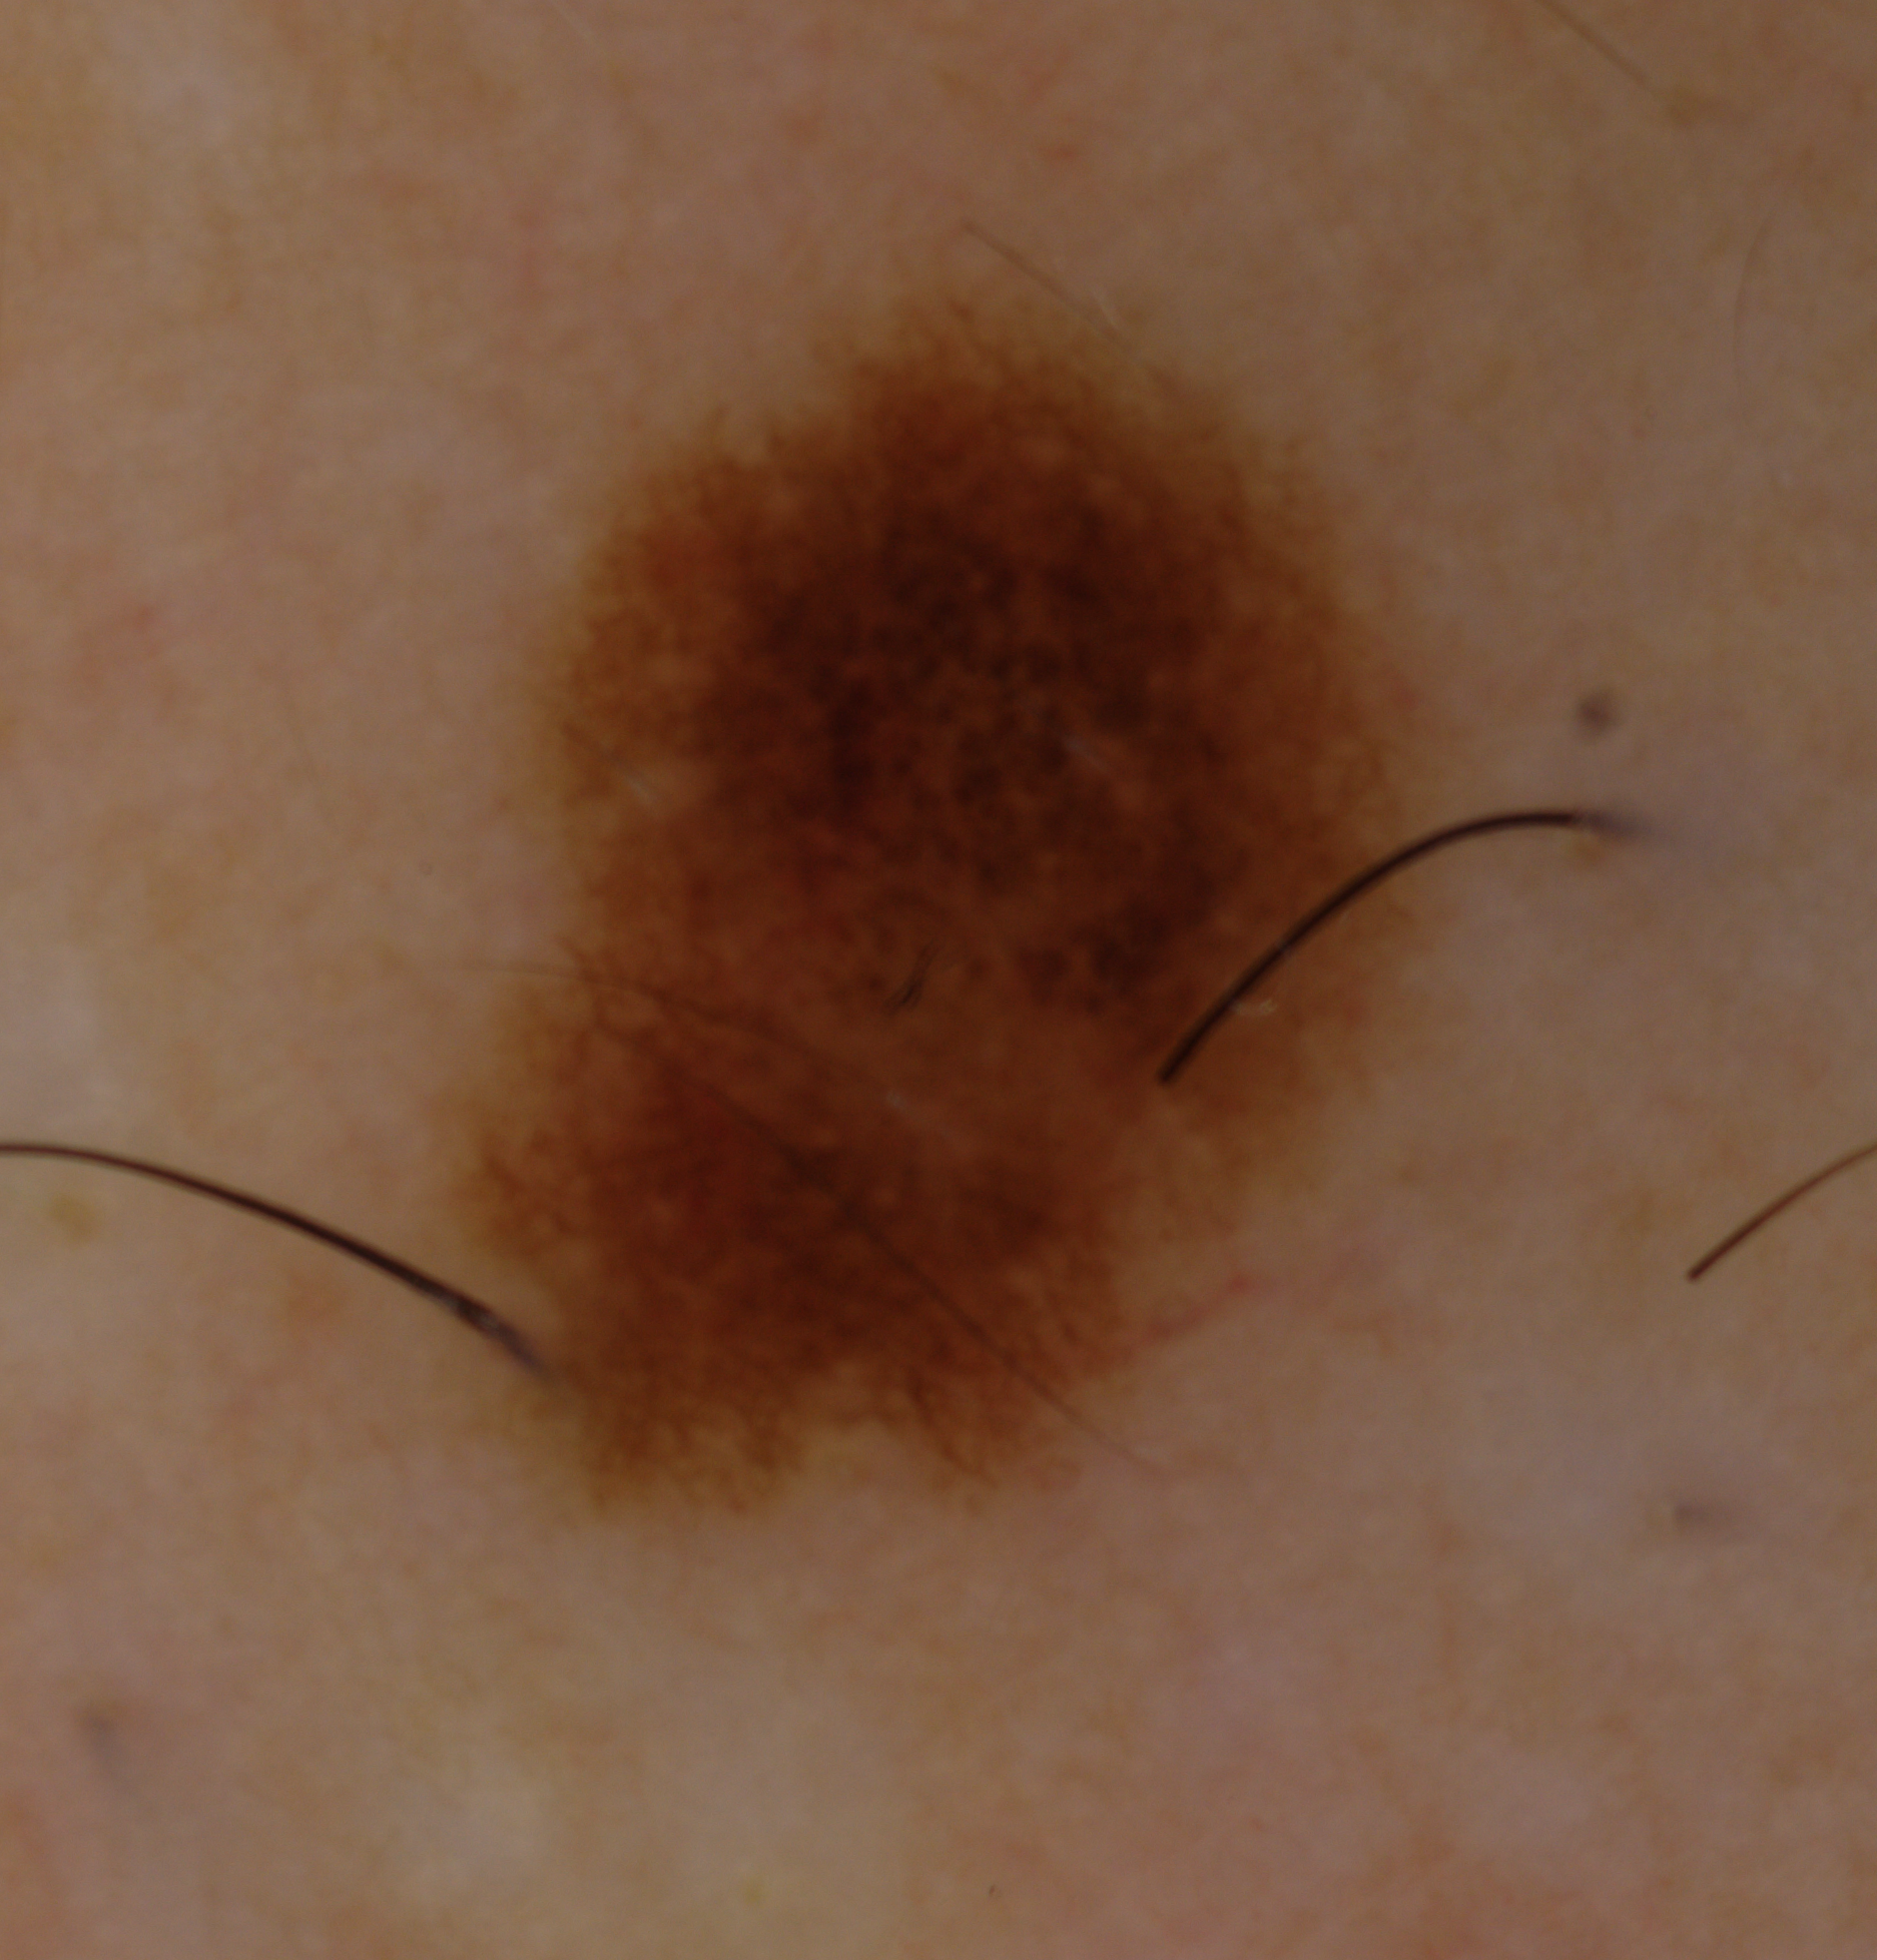
\includegraphics[width = 0.3\textwidth]{Chapter5/Figures/IMG_8443_R.jpg}}\hfill
	\subfloat{\includegraphics[width = 0.3\textwidth]{Chapter5/Figures/HairMask_8443.png}}\hfill
	\subfloat{\includegraphics[width = 0.3\textwidth]{Chapter5/Figures/IMG_8443.png}}\\
	\subfloat{\includegraphics[width = 0.3\textwidth]{Chapter5/Figures/IMG_7110_R.jpg}}\hfill
	\subfloat{\includegraphics[width = 0.3\textwidth]{Chapter5/Figures/HairMask_7110.png}}\hfill
	\subfloat{\includegraphics[width = 0.3\textwidth]{Chapter5/Figures/IMG_7110.png}}\\
	\caption[Examples of hair removal algorithm on polarimetric images]{Hair removal algorithm used on several polarimetric images.}
	\label{fig:hair-removal}
\end{figure}

\subsubsection{Segmentation}
%The segmentation approach was designed specifically for the images acquired by our polarimetric device.
Thanks to having several images of the same lesion with different contrasts, $I_{\ang{0}}$, $I_{\ang{45}}$, and $I_{\ang{90}}$, and a polarimetric image \ac{dolp}, we can apply a rather simple segmentation algorithm: Otsu thresholding~\cite{otsu1975threshold}. 
This algorithm considers that a given image contains two classes of pixels, foreground and background, and attempts to find the intensity threshold that separates the two classes.
The optimum threshold is set so that the within-class variance is minimized.
This method calculates all the possible threshold values and measures pixel characteristics (mean, variance and weights) on each side of the threshold. 
%Characteristics such as mean, variance and weight are then calculated for the two groups of pixels.
Then the within-class variance is calculated for each level, and the level with the minimum within-class variance is considered as the threshold.
%The main goal is to find the threshold value where the sum of foreground and background ranges is at its minimum [19]. 
Equation~\ref{eq:Otsu1} shows how this variance is calculated for two classes in one level:
\begin{equation}
	\sigma_{W}^{2} = W_{b}\sigma_{b}^{2} + W_{f}\sigma_{f}^{2},
	\label{eq:Otsu1}
\end{equation}
\noindent where $W_{b}$ and $W_{f}$ are the weights of the background and foreground, respectively, and $\sigma_{b}$, $\sigma_{f}$ represent the variance of each class.

The computation of the within-class variance can be expensive.
So instead, the between-class variance can be used since its maximization is equivalent to the minimization of the within-class variance~\cite{otsu1975threshold}.
%Instead, the between-class variance can be calculated since maximization of the between-class variance is equivalent to minimization of within-class variance~\cite{otsu1975threshold}.
This computation is shown in Eq.\,\ref{eq:Otsu2}.
\begin{equation}
	\sigma_{B}^{2} = W_{b}W_{f}(\mu_{b}-\mu_{f})^{2},
	\label{eq:Otsu2}
\end{equation}
\noindent where, $\mu_{b}$ and $\mu_{f}$ are the mean of the background and foreground classes, respectively.

Using the Otsu algorithm, the larger area in the segmented image is considered as the main region of interest.
The four segmentations are then combined, and the final lesion mask contains only the areas present in at least three out of the four segmentations.
In addition, the resulting segmentation is optimized using morphological dilation with a disk structuring element of size 2~\si{px}.
Thus, the majority voting on the segmentations obtained from a series of images overcomes the drawbacks of a simple algorithm such as Otsu.

In our approach, three segmentation regions are considered for each lesion: internal, external and their combination (combined).
The internal region is the output of the majority voting after the morphological step.
To obtain the external region, the boundary of the internal segmentation is detected and expanded using the dilation operation with a square of size 50 pixels as the structuring element.
Considering the internal and external segmented regions, the combined segmented area is simply a combination of the two aforementioned regions.
Figure~\ref{fig:segmentation} shows some segmentation results obtained using this approach.

\begin{figure}
	\begin{center}
		\subfloat[]{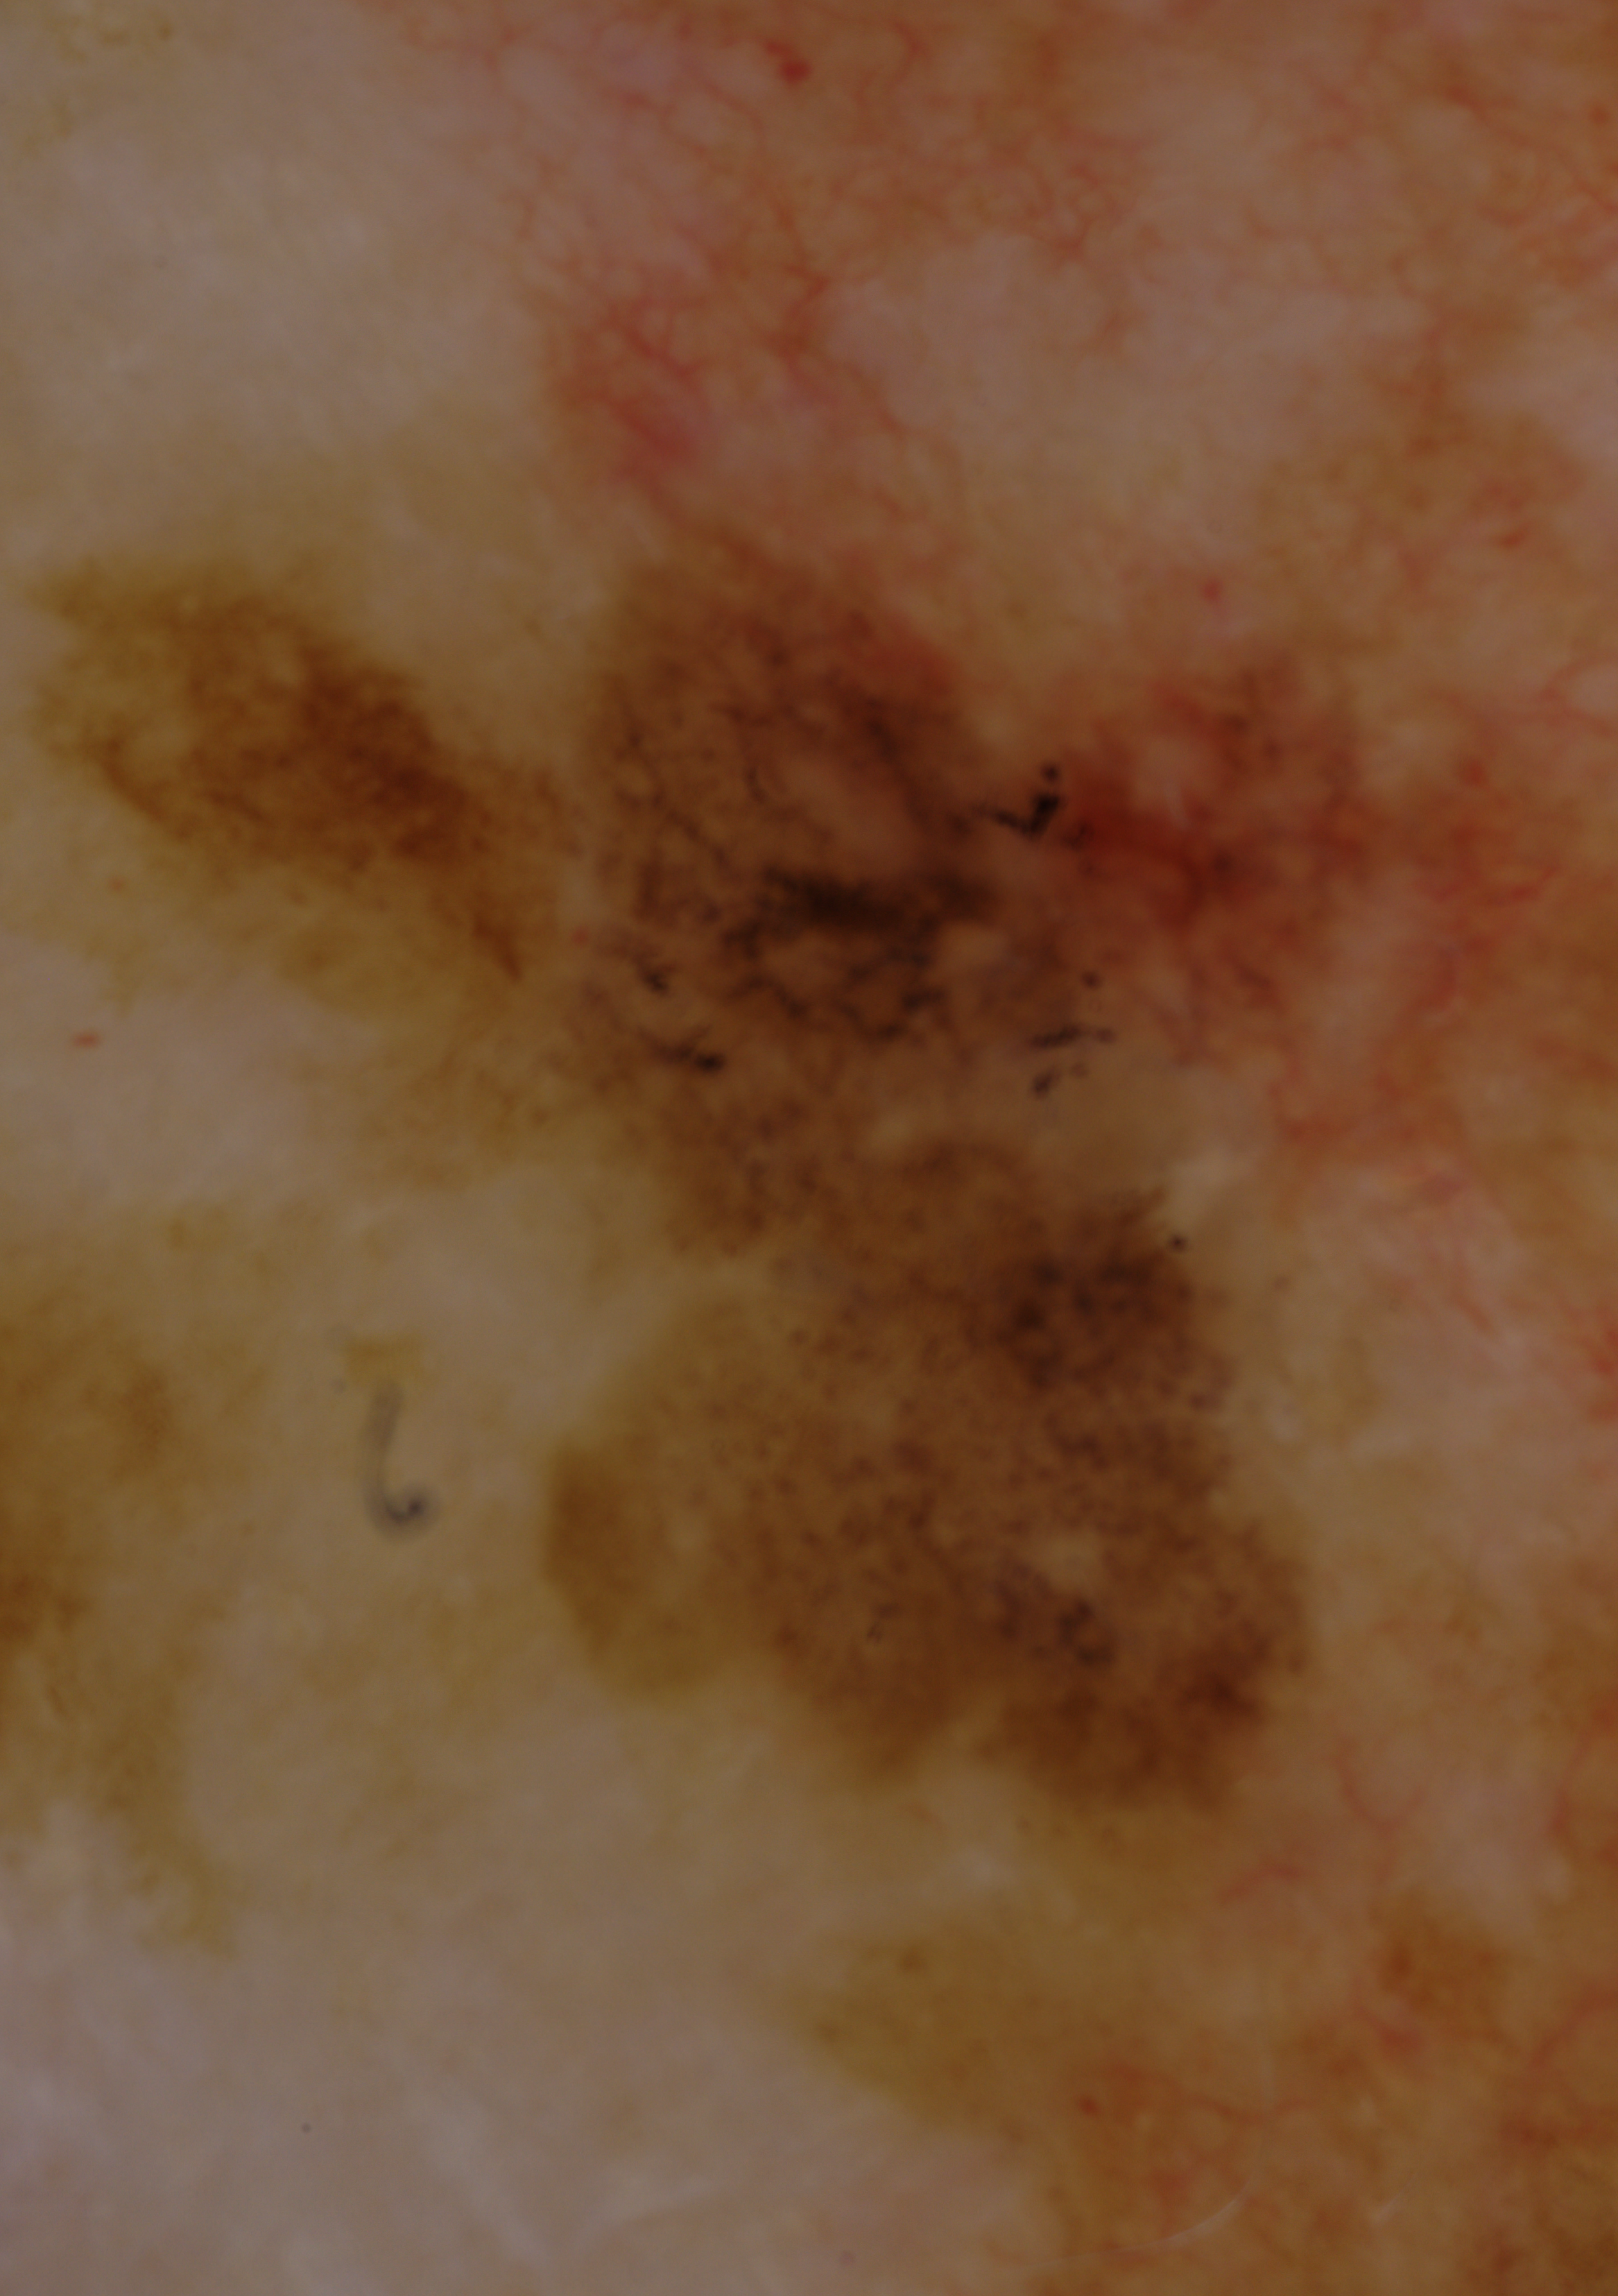
\includegraphics[width = 0.3\textwidth]{Chapter5/Figures/IMG_6646_R.jpg}}\hfill
		\subfloat[]{\includegraphics[width = 0.3\textwidth]{Chapter5/Figures/Mask1_6646.png}}\hfill
		\subfloat[]{\includegraphics[width = 0.3\textwidth]{Chapter5/Figures/Mask2_6646.png}}\\
		\subfloat[]{\includegraphics[width = 0.3\textwidth]{Chapter5/Figures/IMG_7145_R.jpg}}\hfill
		\subfloat[]{\includegraphics[width = 0.3\textwidth]{Chapter5/Figures/Mask1_7145.png}}\hfill
		\subfloat[]{\includegraphics[width = 0.3\textwidth]{Chapter5/Figures/Mask2_7145.png}}\\
		\subfloat[]{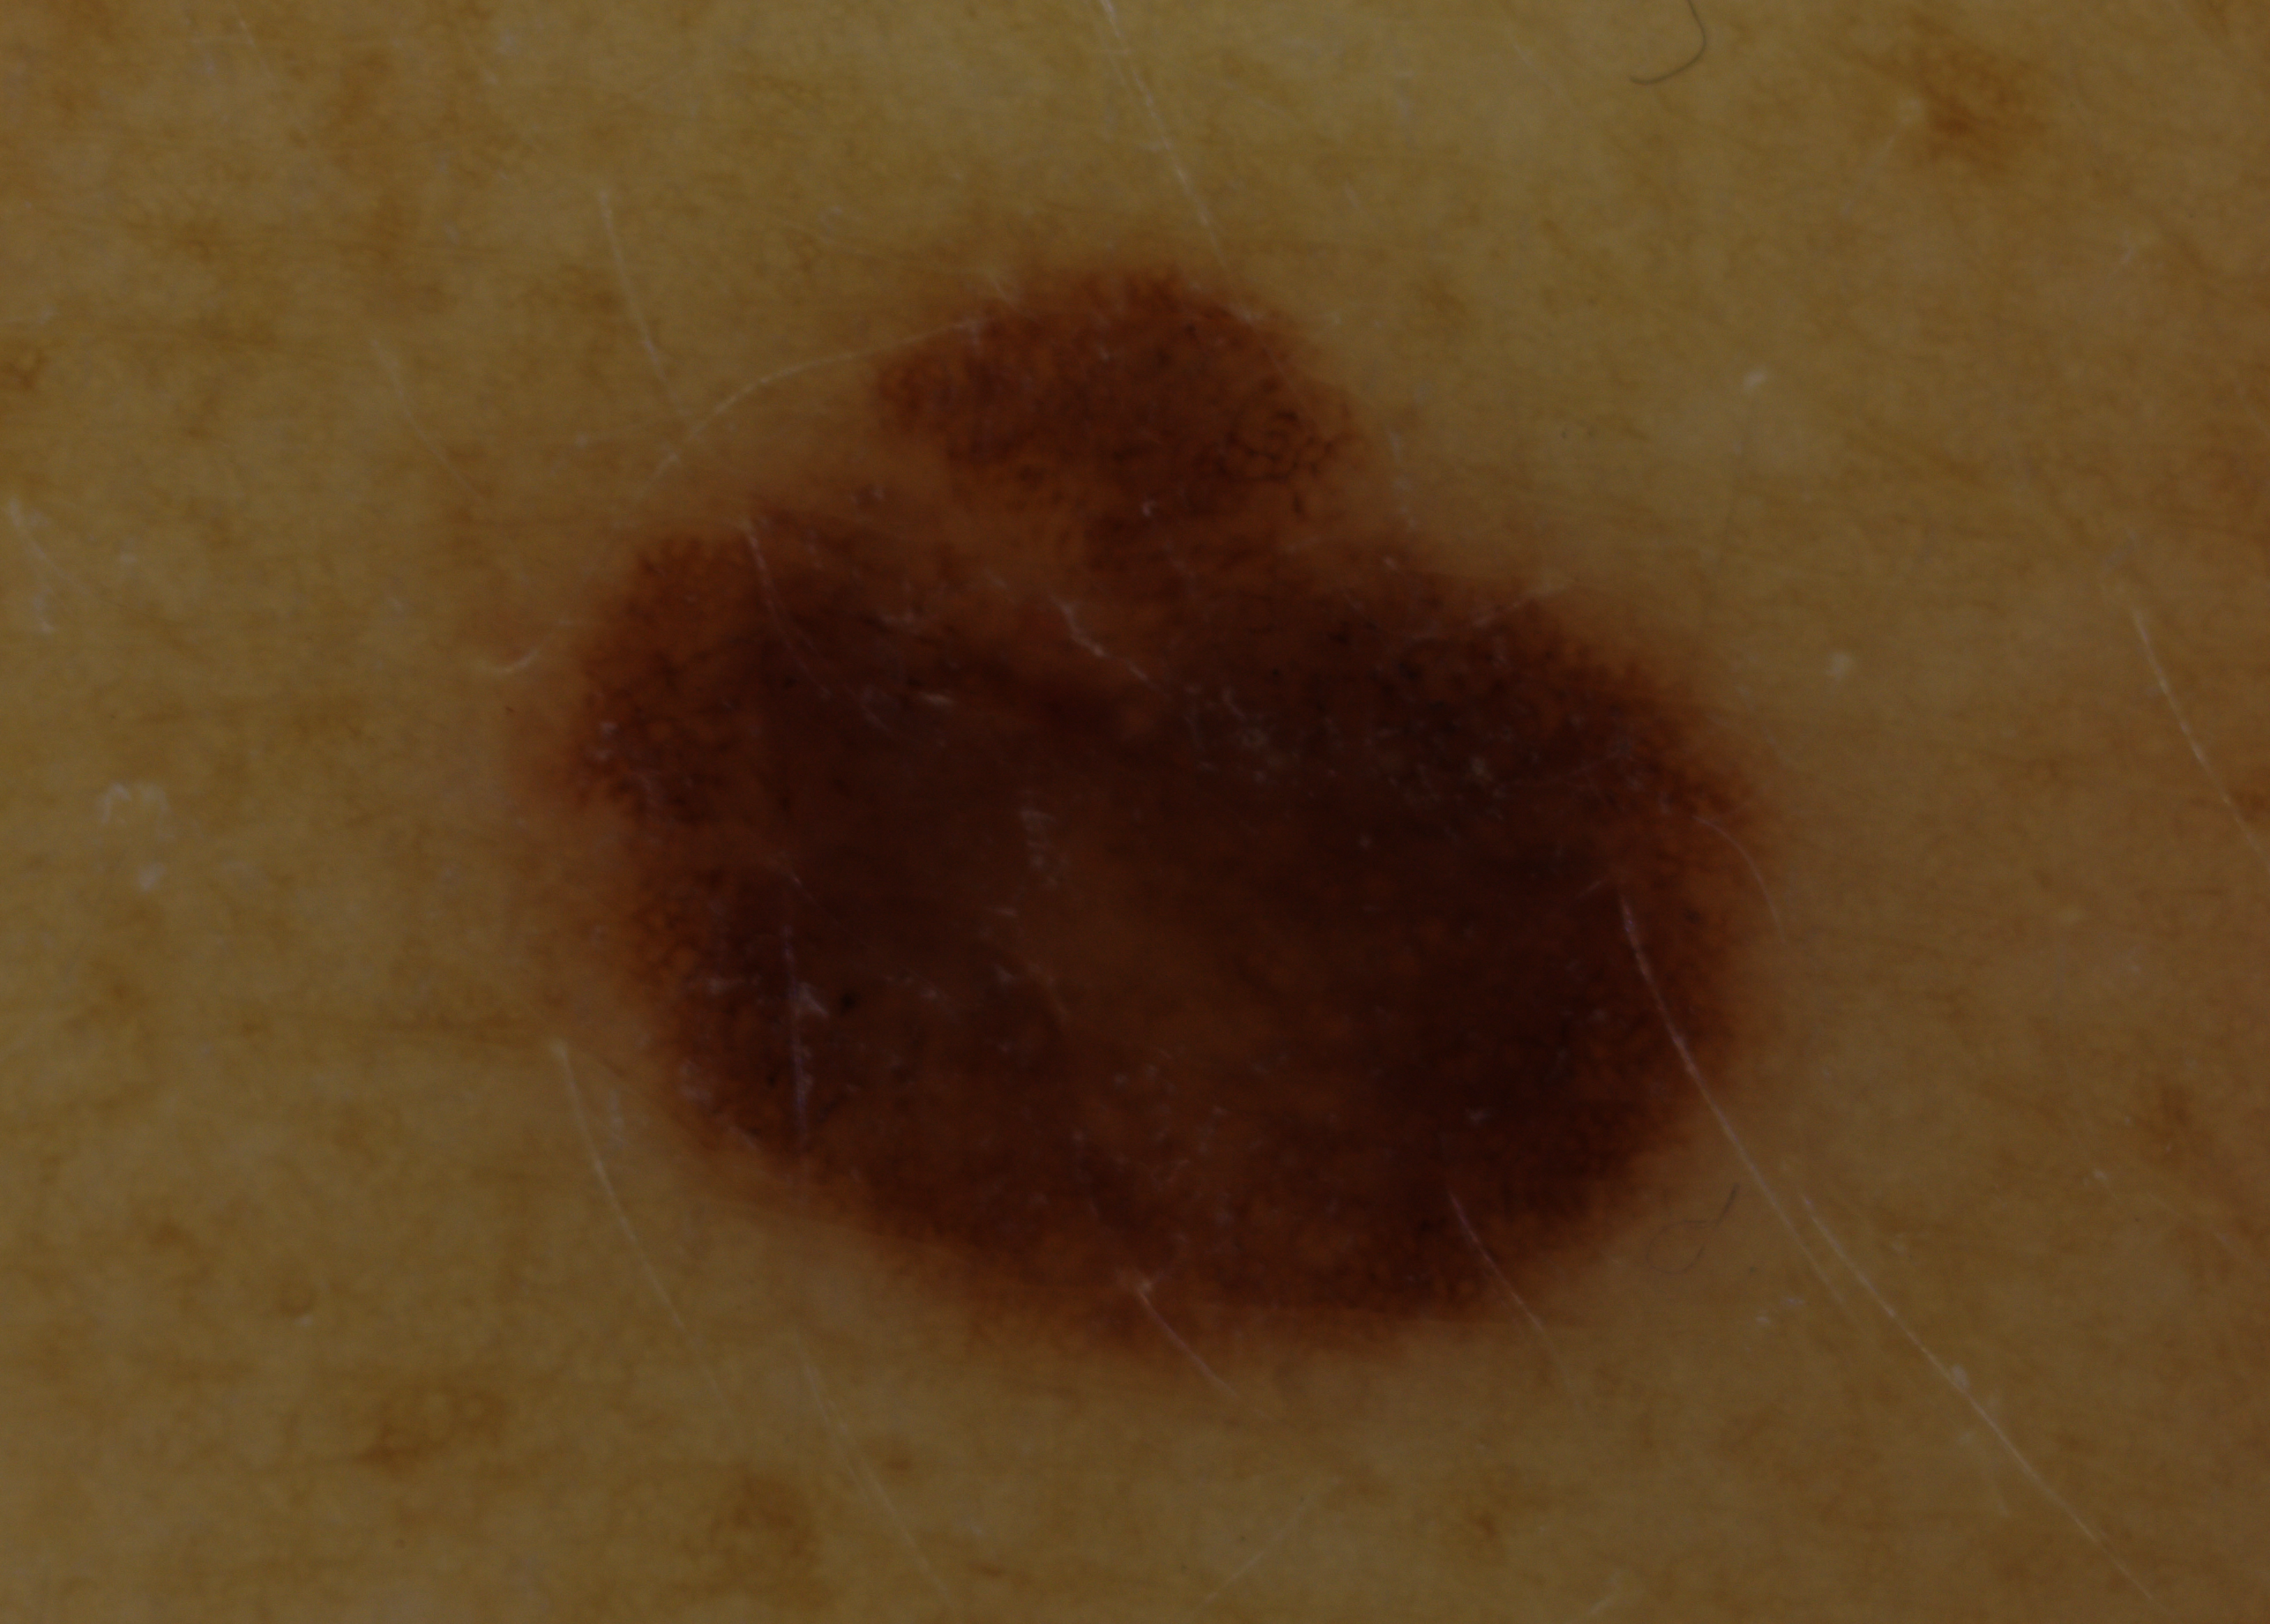
\includegraphics[width = 0.3\textwidth]{Chapter5/Figures/IMG_7032_R.jpg}}\hfill
		\subfloat[]{\includegraphics[width = 0.3\textwidth]{Chapter5/Figures/Mask1_7032.png}}\hfill
		\subfloat[]{\includegraphics[width = 0.3\textwidth]{Chapter5/Figures/Mask2_7032.png}}
	\end{center}
	\caption[Segmentation results on polarimetric images]{Examples of segmentations on polarimetric images of pigmented skin lesions.
	The leftmost column shows the cross-polarized image ($I_{\ang{90}}$) acquired with our device.
	The middle and rightmost columns show the internal and external segmentation regions, respectively.}
	\label{fig:segmentation}
\end{figure}

%-------------------------
\subsection{Mapping}
Since finding the polarimetric properties of the entire lesion is the main goal of this research, we opted for global mapping (see Sect.\,\ref{chp3-subsec2})
Therefore, the features are extracted from either the segmented lesion or the region of interest bound to the lesion's edges.

\subsection{Feature extraction}
Due to the nature of the images, two sets of features were extracted: polarimetric and spatial (dermoscopy) features.
Table~\ref{tab:table2} illustrates a list of descriptors for each category.
The spatial features are those that can be obtained from color dermoscopy images, so they were only extracted from the cross-polarized image ($I_{90}$).
With reference to our previous experiments and the framework for dermoscopy images, two color and four texture features were considered: color statistics ($C_{1}$), opponent angle and hue histogram ($C_{2}$), \acf{clbp} ($T_{1}$), \acf{glcm} ($T_{2}$), Gabor filters ($T_{3}$), and \acf{hog} ($T_{4}$).
These features are extracted from the region of interest bound to the edges of the entire segmented lesion (similar to the global features in the dermoscopy framework).
For the sake of comparison, we used the same extraction parameters.
See Chapter~\ref{chp:chapter3}, Sect.\,\ref{chp3-subsec3} for a detailed explanation of these features.

Polarimetric features, as the name suggests, are extracted from polarimetric images. 
In the current stage of our algorithm, the polarimetric features are extracted from mono-channel inputs, grayscale of I$_{\ang{90}}$, I$_{\ang{45}}$, and I$_{\ang{0}}$.  
After primary observations, we considered using the \ac{dolp}, polarization intensity (Pol$_{~int}$), and the third Stokes parameter $U$.
The last two paramaters are intensity independent, therefore prior to feature extraction the optained images are normalized. 
Equation~\ref{eq:PF} shows the formulation of these parameters once again:
\begin{align}
	\ac{dolp} & = \frac{\sqrt{U^2 + Q^2}}{I}, \\
	\text{Pol}_{~int} & = \sqrt{U^2 + Q^2}, \\
	U & = 2I_{\ang{45}} - I_{\ang{0}} - I_{\ang{90}}. 
	\label{eq:PF}
\end{align}
Figure~\ref{fig:PF-image} shows the images of these parameters for the two melanoma samples.
The polarimetric features are extracted from the segmented area of the lesions.
As explained above, each lesion is segmented into external and internal areas, and therefore, the polarimetric features are extracted for internal, external and combined regions.
The features for external and internal regions are annotated with the extension of $_{E}$ and $_{I}$, respectively.

\begin{figure}
	\begin{center}
		\captionsetup[subfigure]{labelformat=empty}
		%\subfloat[$I_{\ang{90}}$]{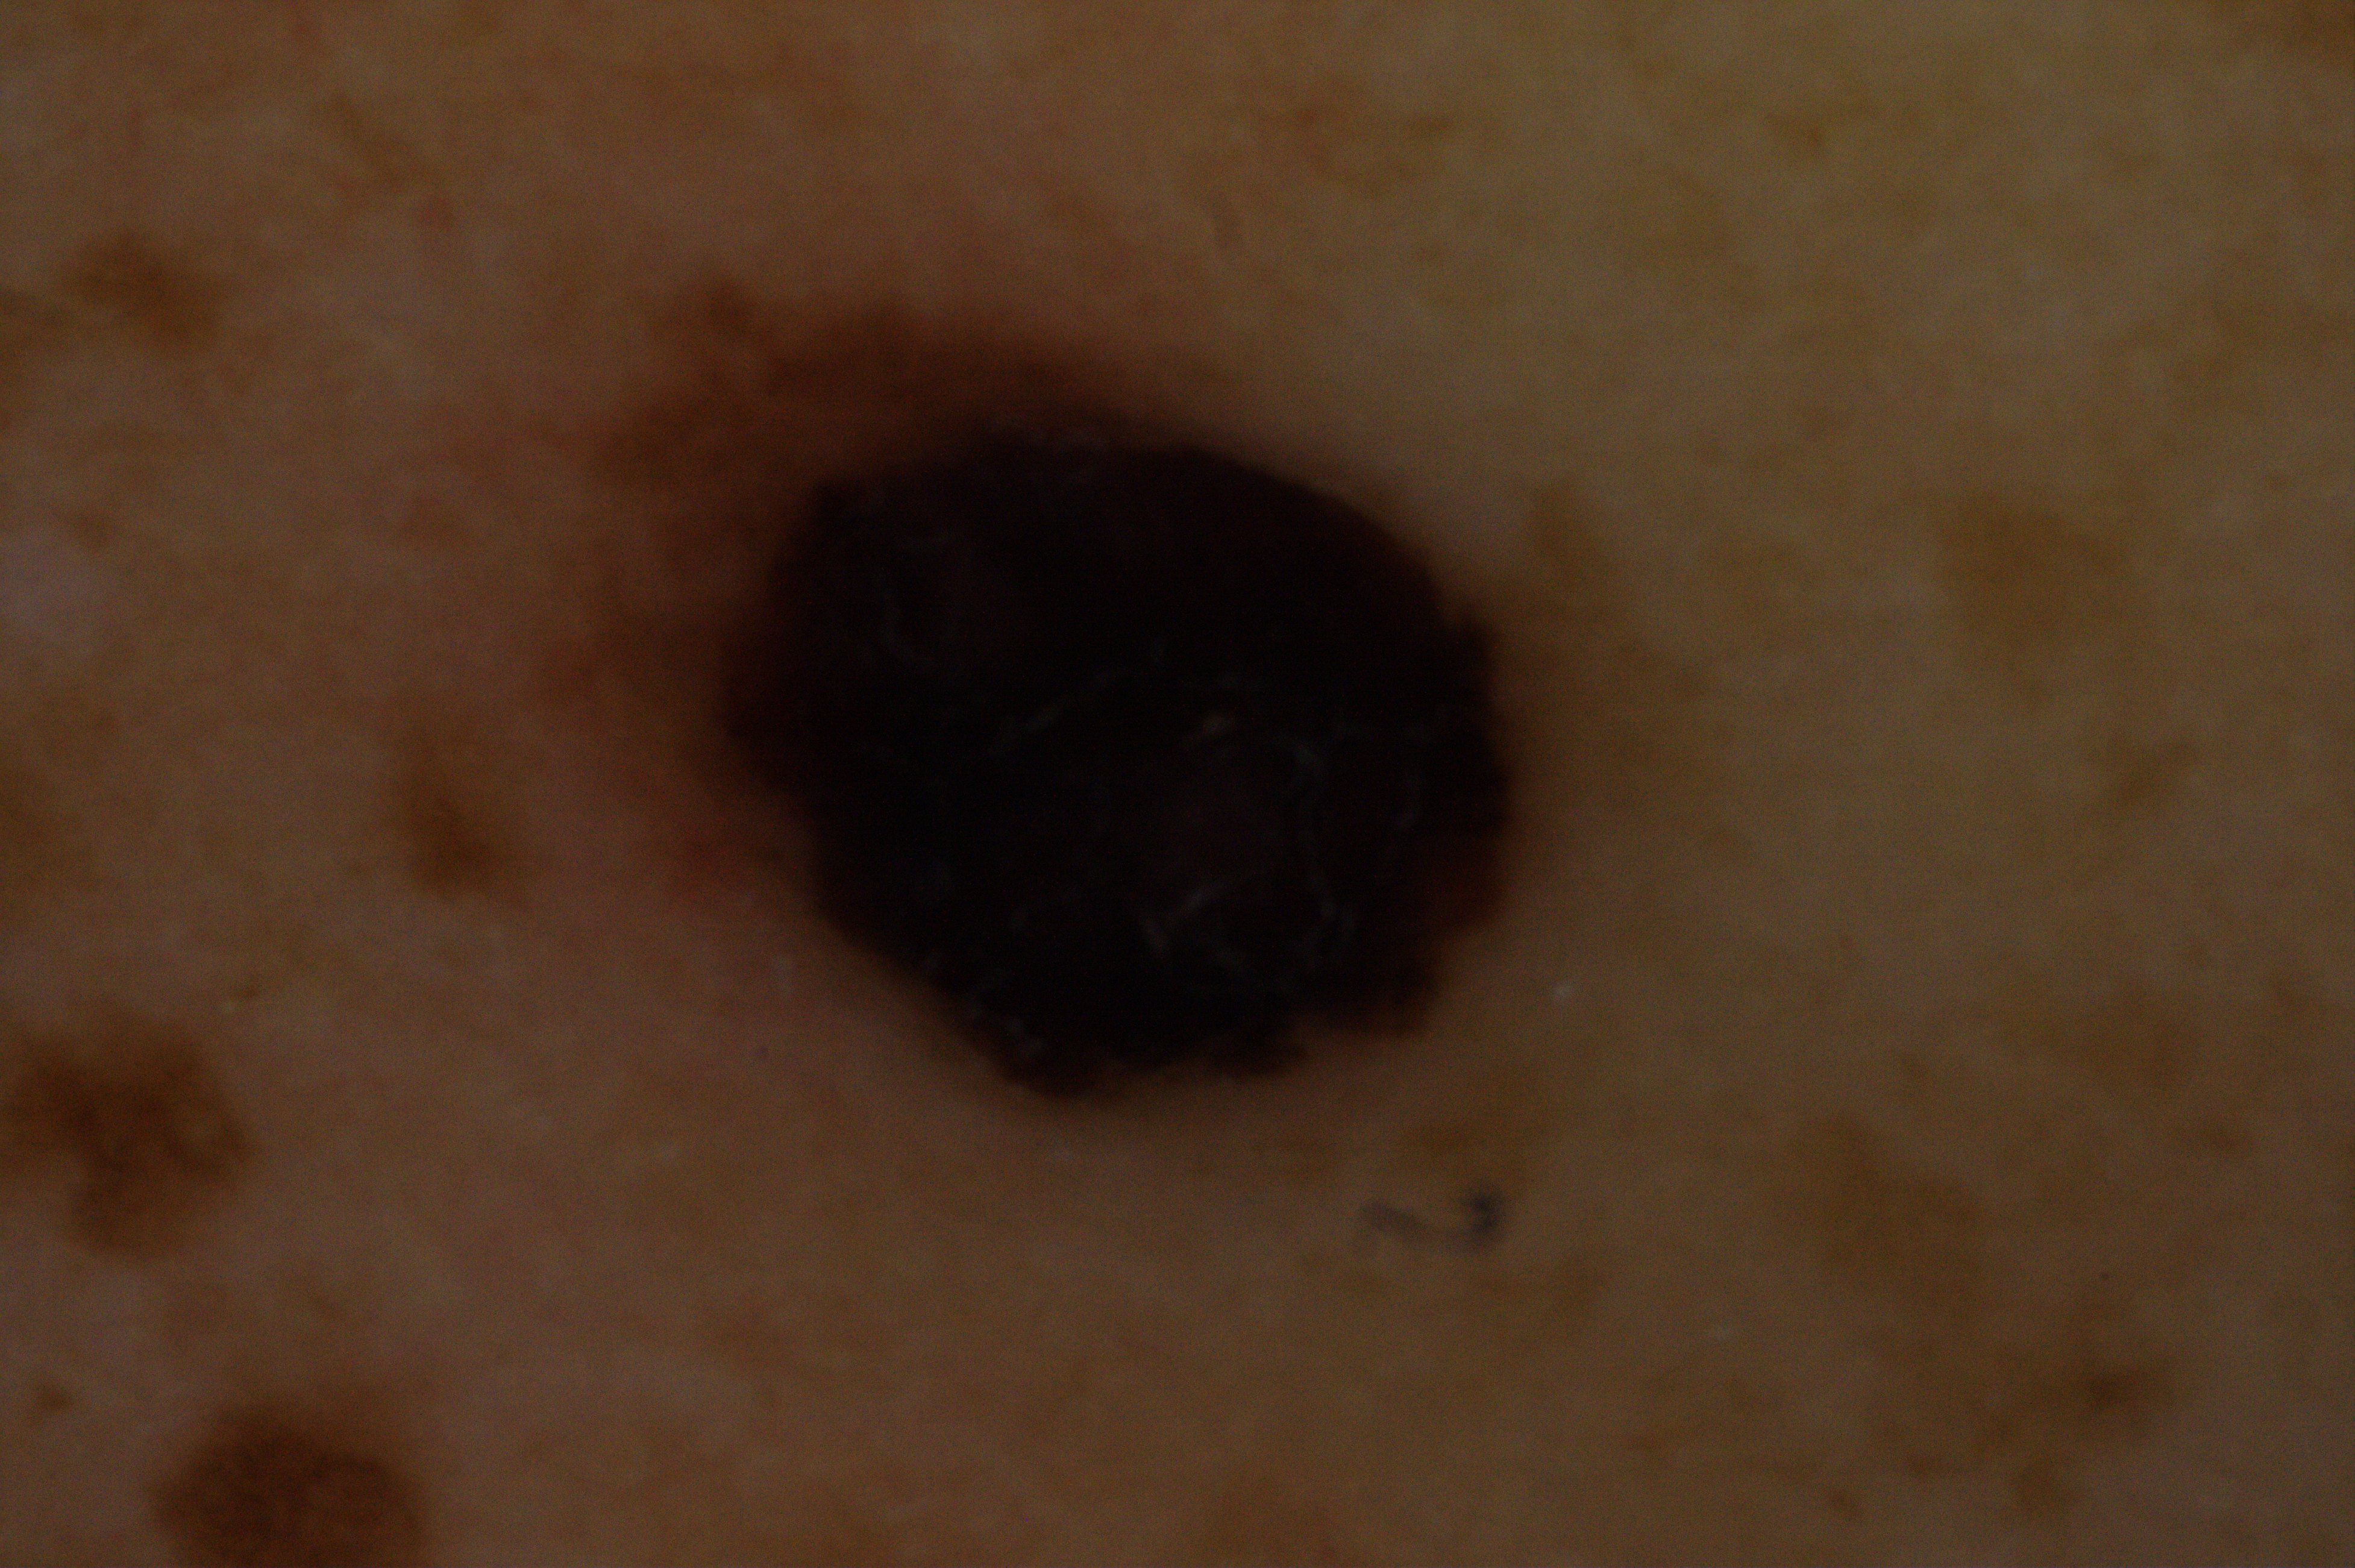
\includegraphics[width = 0.4\textwidth]{Chapter5/Figures/IMG_6561_R.png}}\hfill
		\subfloat[\ac{dolp}]{\includegraphics[width = 0.45\textwidth]{Chapter5/Figures/IMG_6561_DoP_Colorbar.png}}\
		\subfloat[\ac{dolp}]{\includegraphics[width = 0.45\textwidth]{Chapter5/Figures/IMG_6890_DoP_Colorbar.png}}\\
		\subfloat[Pol$_{~int}$]{\includegraphics[width = 0.45\textwidth, height = 0.205\textheight]{Chapter5/Figures/IMG_6561_Polint_Colorbar.png}}\
		\subfloat[Pol$_{~int}$]{\includegraphics[width = 0.45\textwidth]{Chapter5/Figures/IMG_6890_Polint_Colorbar.png}}\\
		\subfloat[U]{\includegraphics[width = 0.45\textwidth]{Chapter5/Figures/IMG_6561_U_Colorbar.png}}\
		%\subfloat[$I_{\ang{90}}$]{\includegraphics[width = 0.4\textwidth]{Chapter5/Figures/IMG_6890_R.png}}\hfill
		\subfloat[U]{\includegraphics[width = 0.45\textwidth]{Chapter5/Figures/IMG_6890_U_Colorbar.png}}
	\end{center}
	\caption[Images of polarimetric features.]{Images of polarimetric features for two melanoma lesions: \ac{dolp}, Pol$_{~int}$, and U.}
	\label{fig:PF-image}
\end{figure}

% Table2 
\begin{table}
\caption[Features used in the automatic classification of melanoma lesions from polarimertic images]{Summary of the features used in the automatic classification of melanoma from polarimetric images.}
\begin{center}
\small{
\resizebox{1\textwidth}{!}{
\begin{threeparttable}
\begin{tabular}{l r}
\toprule
\multicolumn{2}{c}{\textbf{Spatial Features}}\\
\midrule
Feature & Index \\
\midrule
\multicolumn{2}{l}{Color} \\
     \quad Color mean and variance along RGB, HSV and LAB & \multirow{2}{*}{$C_{1}$}\\
     \quad Color histogram in RGB (\textit{b = 42} ) \tnote{1} & \\
     \quad Opponent color space angle and hue histogram (\textit{b = 42}) & $C_{2}$\\ 
\multicolumn{2}{l}{Texture} \\
	\quad Completed Local Binary Pattern \tnote{2}& $T_{1}$\\
	\quad Gray-Level Co-occurrence Matrix ($\theta$ = \{$0$, $\pi/4$, $\pi/2$, $3\pi/4$\}, \textit{D = 9 pxls}, \textit{G = 32})\tnote{3} & $T_{2}$ \\
    \quad Gabor Filter (s = 4 , $\theta$= \{$\pi/6$, $\pi/3$, $\pi/2$, $2\pi/3$, $5\pi/6$, $\pi$\}) & $T_{3}$ \\
    \quad Histogram of Oriented Gradients & $T_{4}$\\
\midrule
\multicolumn{2}{c}{\textbf{Polarimetric Features}}\\
\midrule
Feature & Index \\
\midrule
\multicolumn{2}{l}{\acs{dolp}}\\
	\quad Histogram of internal segmentation & $D_{H_{I}}$\\
	\quad Histogram of external segmentation & $D_{H_{E}}$\\
	\quad Histogram of segmented lesion & $D_{H}$\\
	\quad Moments of internal segmentation & $D_{M_{I}}$\\
	\quad Moments of external segmentation & $D_{M_{E}}$\\
	\quad Moments of segmented lesion & $D_{M}$\\
\multicolumn{2}{l}{Pol$_{~int}$}\\
	\quad Histogram of internal segmentation & $P_{H_{I}}$\\
	\quad Histogram of external segmentation & $P_{H_{E}}$\\
	\quad Histogram of segmented lesion & $P_{H}$\\
	\quad Moments of internal segmentation & $P_{M_{I}}$\\
	\quad Moments of external segmentation & $P_{M_{E}}$\\
	\quad Moments of segmented lesion & $P_{M}$\\
\multicolumn{2}{l}{U}\\
	\quad Histogram of internal segmentation & $U_{H_{I}}$\\
	\quad Histogram of external segmentation & $U_{H_{E}}$\\
	\quad Histogram of segmented lesion & $U_{H}$\\
	\quad Moments of internal segmentation & $U_{M_{I}}$\\
	\quad Moments of external segmentation & $U_{M_{E}}$\\
	\quad Moments of segmented lesion & $U_{M}$\\
	\quad Magnitude of gradients & $U_{Gmag}$\\
\bottomrule




%\midrule


\end{tabular}
  \scriptsize{
  \begin{tablenotes}
  \item[1] \textit{b} stands for the number of bins.
  \item[2] 24 neighbourhood, rotation invariant, uniform and normalized histogram.
  \item[3] \textit{D} stands for distance in pixels and \textit{G} is the quantized number of gray levels.
  \end{tablenotes}
  }
\end{threeparttable}}}
\end{center}
\label{tab:table2}
\end{table}


\subsection{Feature representation}
The primary objective of the proposed classification  framework is to evaluate the polarimetric features in comparison with their spatial counterparts.
Thus, we considered the simplest forms of feature representation.
The \ac{dolp}, Pol$_{~int}$, and U features were characterized by (i) histograms and (ii) statistical moments (mean, standard deviation, skewness, and kurtosis) of the polarimetric feature distribution.
The representations based on histograms and moments are denoted in Table~{\ref{tab:table2}} with the extensions $_H$ and $_M$, respectively.
The U feature was also represented by the magnitude of gradients ($U_{Gmag}$).
The gradient of the gray image is obtained by convolving the image with the Sobel mask in the horizontal and vertical directions. 
By doing so, a gradient vector for each point is obtained ($[G_{x} \quad G_{y}]^{T}$), from which the gradient magnitude ($G$) and phase ($\theta$) are calculated using the following formulation (here, only the gradient magnitude is used):
\begin{align}
	\Vert G(x) \Vert & = \sqrt{G_{x}^2(x) + G_{y}^{2}(x)}, \\
	\theta(x) & =  atan2(G_{y}(x), G_{x}(x)).
	\label{eq:MPgrad}
\end{align}

\subsection{Balancing}
As illustrated in Table~\ref{tab:table1}, our polarimetric dataset is imbalanced. 
In order to reduce the effect of the imbalance problem, prior to classification, over and under-sampling techniques in the feature space are applied.
The same techniques, previously explained in Sect.\,\ref{sec:chp2-sec5}, are used here as well: \ac{ros}, \ac{smote}, \ac{rus}, \ac{cus}, \ac{ncr}, \ac{nm1}, \ac{nm2}, \ac{nm3}, \ac{tl}, \ac{smote}+\ac{enn}, and \ac{smote}+\ac{tl}.

\subsection{Classification}
In this framework, the only classifier we applied was the \acl{rf} ensemble.
This decision was made based on the quantitative results obtained in the experiments with the classification framework for dermoscopy images, where the RF ensemble showed the best results.
%This classifier is trained with 100 un-prunned trees in the following experiments.
